\newpage

\section{Midterm 2 Review Problems}

\begin{prob}
During a solar eclipse we see that the apparent diameter of the Sun and Moon are nearly equal. If the Moon is around 240,000 miles from Earth, the Moon's diameter is about 2000 miles, and the Sun's diameter is about 865,000 miles how far is the Sun from the Earth?
\begin{enumerate}
\item Draw a relevant (and helpful) picture showing the important points of this problem.
\item Write an expression that gives the solution to this problem---show all work.
\end{enumerate}
\end{prob}

\begin{prob}
A typical adult male gorilla is about 5.5 feet tall and weighs about 400 pounds. Suppose King Kong was about 22 feet tall and proportioned like a typical adult male gorilla.
\begin{enumerate}
\item Write an expression that approximates King Kong's weight. Briefly explain your reasoning.
\item The circumference of the neck of a typical adult male gorilla is 36 inches. Approximately what would be the circumference of King Kong's neck? Briefly explain your reasoning.
\item Suppose an Ohio State sweatshirt for a typical adult male gorilla requires 3 square yards of fabric.  Approximately how much fabric would be required for an Ohio State sweatshirt for King Kong?  Briefly explain your reasoning.
\end{enumerate}
\end{prob}

\begin{prob}
Brenah is drinking fruit punch from a glass shaped like an inverted cone.  Suppose the glass has a height 5 in. and a base of radius 2 in.  What is the volume of the glass?  What is the height of the fruit punch when the glass is half full?  Generalize your result for any glass shaped like an inverted cone.  
\end{prob}

\begin{prob}
A cup has a circular opening, a circular base, and circular cross sections at every height parallel to the base.  The opening has a diameter of 9 cm, the base has a diameter of 6 cm, and the cup is 12 cm high.  
What is the volume of the cup?  Explain your reasoning.  
If the cup is filled to half its height, what fraction of the cup's volume is filled?  Explain your reasoning.  
\end{prob}

\begin{prob}
Suppose you use a photocopier to enlarge a figure to 125\% of its original size.  What is the scale factor of the enlargement?  What happens to areas under the enlargement?  If you lost the original figure, what reduction percentage would you use on the enlargment to create a figure congruent to the original?  What is the scale factor for the reduction?  
\end{prob}

\begin{prob}
Explain how the following picture ``proves'' the Pythagorean Theorem.
\[
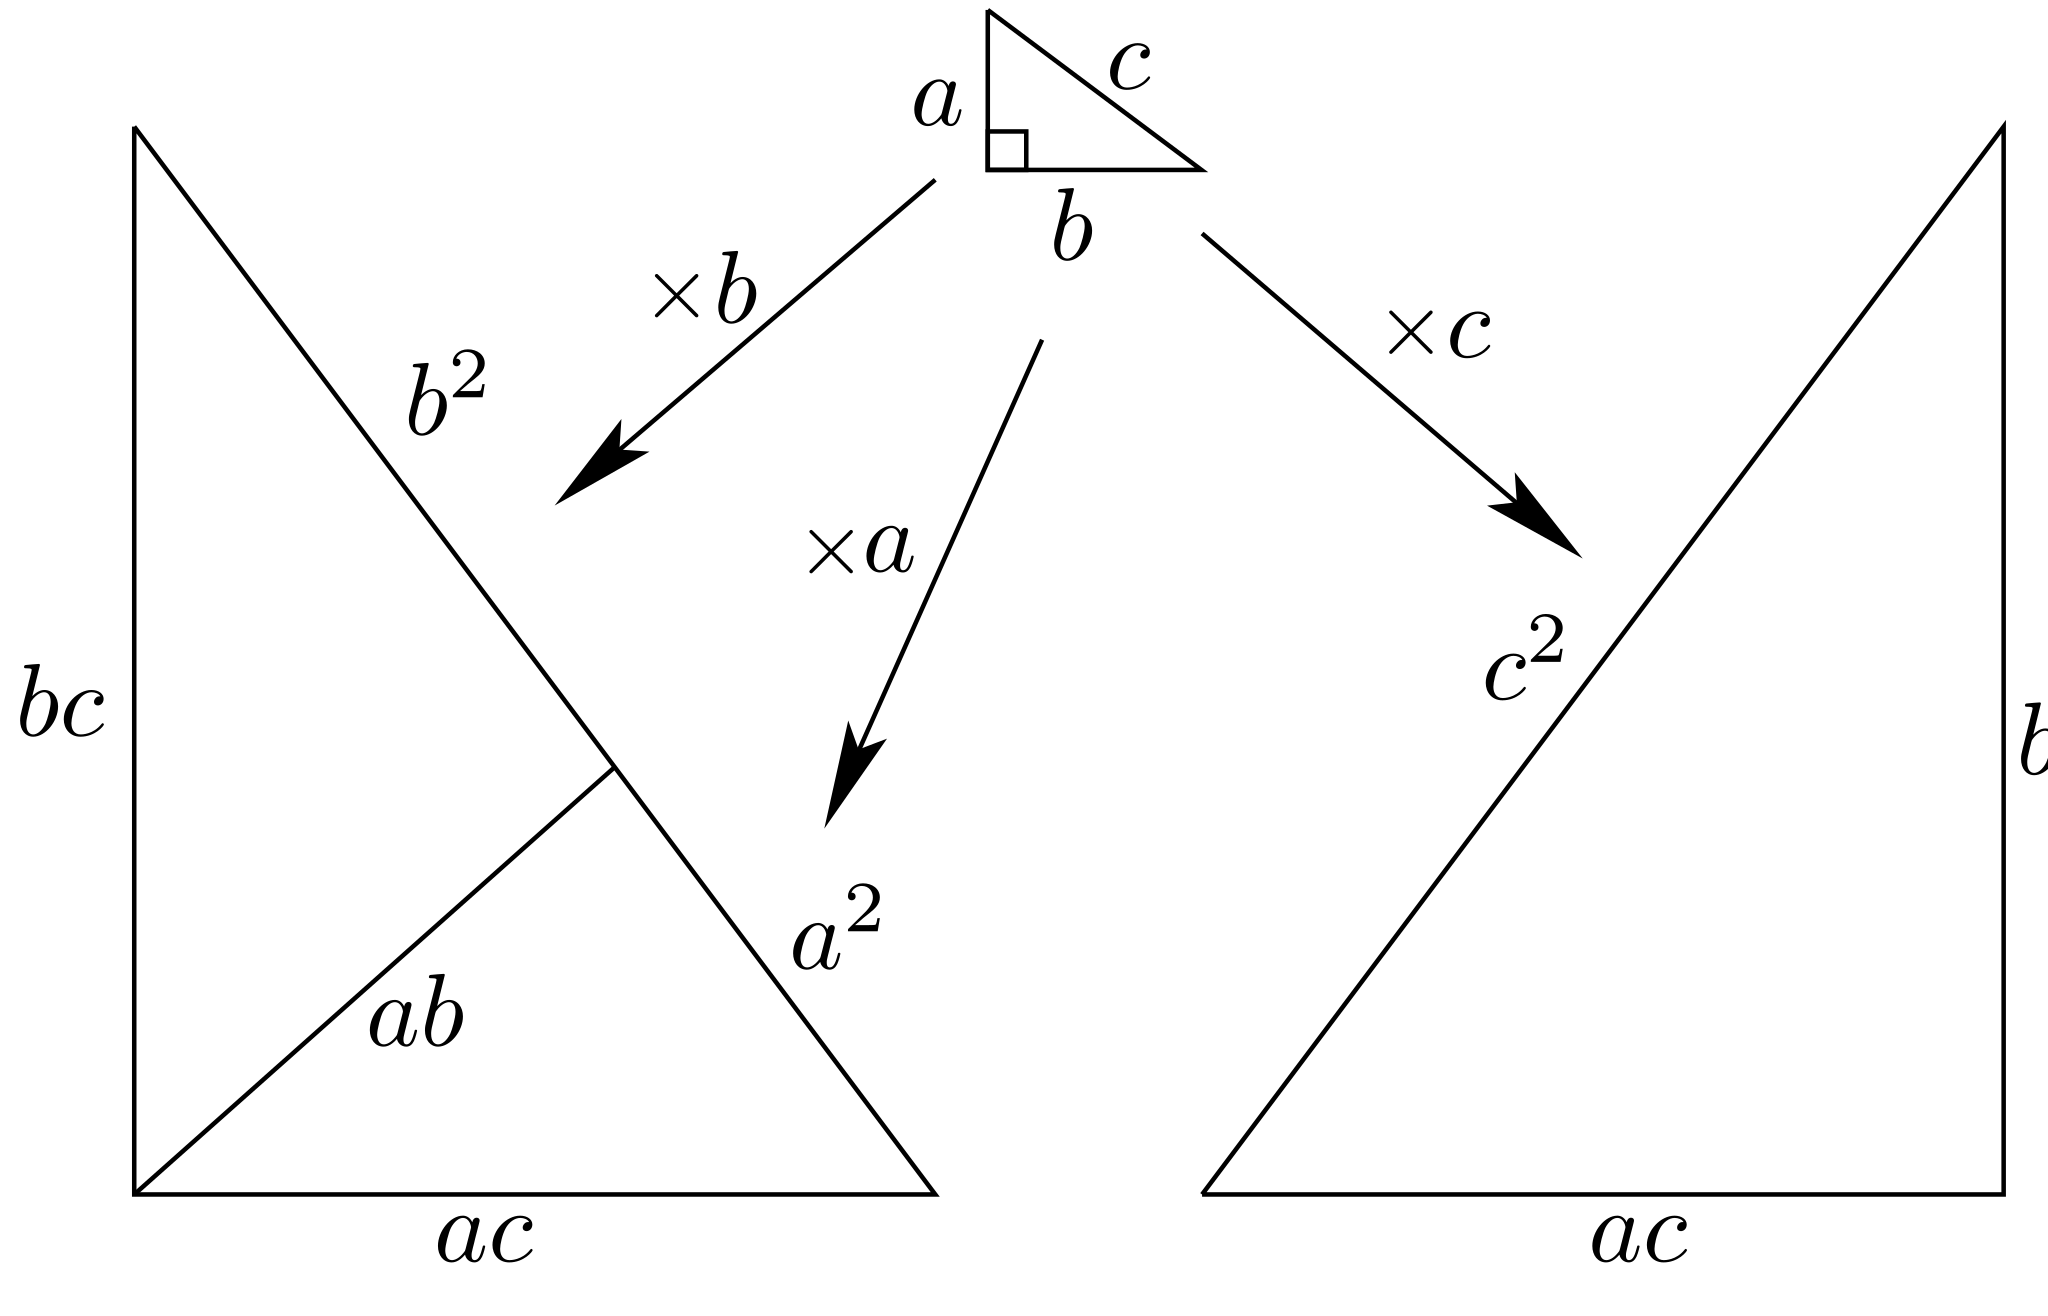
\includegraphics[scale=0.8]{../graphics/pbpdilation.pdf}
\]
\end{prob}

\begin{prob}
Here is a right triangle, note it is \textbf{not} drawn to scale:
\[
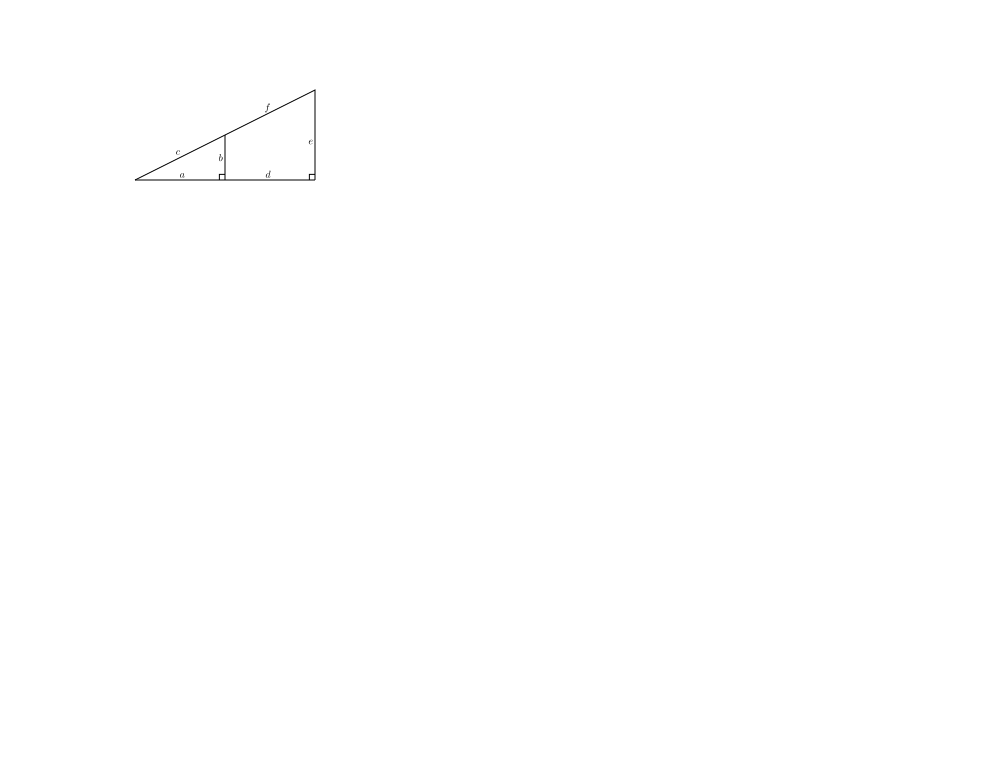
\includegraphics{../graphics/origamiSimQ.pdf}
\]
Solve for all unknowns in the following cases.
\begin{enumerate}
\item $a = 3$, $b = ?$, $c = ?$, $d = 12$, $e = 5$, $f = ?$
\item $a = ?$, $b = 3$, $c = ?$, $d =8$, $e = 13$, $f = ?$
\item $a = 7$, $b = 4$, $c = ?$, $d =?$, $e = 11$, $f = ?$
\item $a = 5$, $b = 2$, $c = ?$, $d =6$, $e = ?$, $f = ?$
\end{enumerate}
In each case explain your reasoning.
\end{prob}

\begin{prob}
Describe a general (and foolproof) way of demonstrating that any two parabolas are similar.
\end{prob}

\begin{prob}
Prove that the angle sum of a triangle is $180^\circ$.
\end{prob}

\begin{prob}
Construct a tangent line from a point outside a given circle to the circle.
\end{prob}

\begin{prob}
Explain how the formula for the volume of a sphere follows from the formula for the volume of a cone and Cavalieri's Principle.
\end{prob}

\begin{prob}
Give an informal derivation of the relationship between the circumference and area of a circle. 
\end{prob}

\begin{prob}
Given a figure and a rotation of that figure, find the center and angle of rotation.  
\end{prob}

\begin{prob}
In the figure below  $O$ is the center of the circle, $\overline{XY}$ is a diameter, $a = PX$, $b=PY$, and $c=PZ$.  
$$\includegraphics[scale=0.7]{Means}$$
\begin{enumerate}
\item Show that $c=\sqrt{ab}$.  
\item Then use the figure to explain the Arithmetic-Geometric Mean Inequality: 
$$\frac{a+b}{2} \ge \sqrt{ab}$$
\item Why is this called the Arithmetic-Geometric Mean Inequality?  
\end{enumerate}
\end{prob}



